\vspace{-0.05in}
\section{Introduction}
\label{sec:intro}
\vspace{-0.05in}

\IEEEPARstart{L}{arge} Language Models (LLMs)~\cite{hurst2024gpt,liu2024deepseek,TPAMI2025LLM_Memristor} empower advanced applications such as multi-turn dialogue~\cite{yi2402survey,teng2024fine,ma2024multi}, long-form document summarization~\cite{zhang2023enhancing,liu2023learning}, and multimodal tasks~\cite{tu2023unsupervised,liu2023visual,lin2023video,tu2025global,TPAMI2025LLM_MultiModal,tu2025automatic} involving text and visual understanding \cite{TPAMI2025LLM_VQA,TPAMI2025LLM_Creativity,tu2025multimodal,TPAMI2025LLM_Disease,lan2025survey,tu2025mllm}. %However, autoregressive decoding maintains a per-layer key–value (KV) cache whose size grows with the generated sequence length $L$, forcing each new query to read increasingly many past KVs. 
However, in autoregressive decoding, the per-layer key–value (KV) cache grows linearly with the generated length $L$, requiring each new query to access an increasingly large set of past KVs.
With $H$ heads and per-head dimension $d$, the per-query attention cost (score computation and value aggregation) scales as $\mathcal{O}(HLd)$~\cite{vaswani2017attention}. As $L$ increases, runtime becomes dominated by attention computation rather than model forward passes; %for example, generating a 40k-token sequence with LLaMA-3.1-8B~\cite{touvron2023llama} entails tens of TFLOPs of attention per step.
for example, at a 40k-token context, LLaMA-3.1-8B~\cite{touvron2023llama} incurs attention compute on the order of tens of TFLOPs per decoding step.

KV compression alleviates these costs by exploiting attention sparsity~\cite{wang2020linformer,sun2025vorta,zhang2023h2o,xiao2023streamingllm}: most KV entries receive negligible attention, so retaining a small, critical subset can approximate full attention while reducing memory traffic and latency. With a per-head budget $k\!\ll\!L$, the top-$k$ oracle retains the $k$ highest-score entries per query, minimizing approximation error and achieving the best accuracy. While this reduces value aggregation from $\mathcal{O}(HLd)$ to $\mathcal{O}(Hkd)$, identifying the top-$k$ still requires computing all scores at $\mathcal{O}(HLd)$ plus a retrieval overhead. Thus, end-to-end cost remains dominated by full scoring, making the oracle impractical for deployment.

To simplify full scoring, existing approaches approximate the top-$k$ oracle by summarizing observed (posterior) attention statistics into priors that constrain future retrieval, yielding posterior-conditioned policies. For example, \emph{Token Dropping Oracles} (TDOs) apply static or dynamic eviction policies~\cite{zhang2023h2o,xiao2023streamingllm,he2024zipcache,wan2024d2o} to keep only entries deemed critical at the current step, restricting the candidate set and reducing per-step scoring to $\mathcal{O}(Hkd)$. \emph{Query-Aware Approximations} (QAAs)~\cite{tang2406quest,sun2024shadowkv,wu2024tokenselect,liu2024hashevict} construct low-dimensional, hand-designed surrogate features to approximate attention scores and use them to guide retrieval, incurring $\mathcal{O}(HLd')$ with $d'\!\ll\!d$.


Despite the efficiency gains, these posterior-driven simplifications incur systematic bias that degrade generative performance.
Specifically, in TDO, token salience evolves over time. Thus, selectors that
condition on observed attention along the trajectory face
non-stationary evidence and systematically skew future decisions
\cite{wan2024d2o,sun2024shadowkv}. In addition, QAAs that
replace full logits with heuristic proxies induce a score-level bias.
We group these archetypes under \textbf{Post-hoc Sparsity (PoHS)}—
\emph{posterior-conditioned} rules that bias token-importance estimates and thereby impair long-range reasoning. Empirically, PoHS yields substantially larger perturbations at both the attention and the output (latent) levels
than the top-$k$ oracle (Fig.~\ref{fig:teaser_attn_diff}, \ref{fig:teaser_latent_diff}; lower is better).

\begin{figure*}[!t]
  \centering
  \captionsetup[subfloat]{font=scriptsize}
  \subfloat[Introduced attention disturbances (absolute difference) after filtering pre-softmax attention logits $\!<\!0$.]{
  \footnotesize
  \label{fig:teaser_attn_diff}
    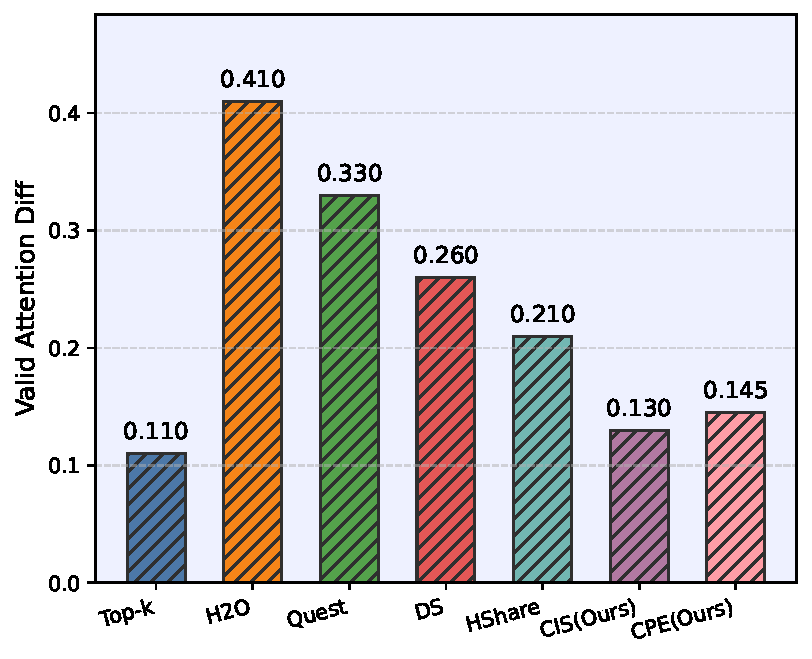
\includegraphics[width=0.305\textwidth]{assets/teaser/attn_diff.pdf}
  }\hfill
  \subfloat[Introduced absolute differences between original attention outputs.]{
  \footnotesize
  \label{fig:teaser_latent_diff}
    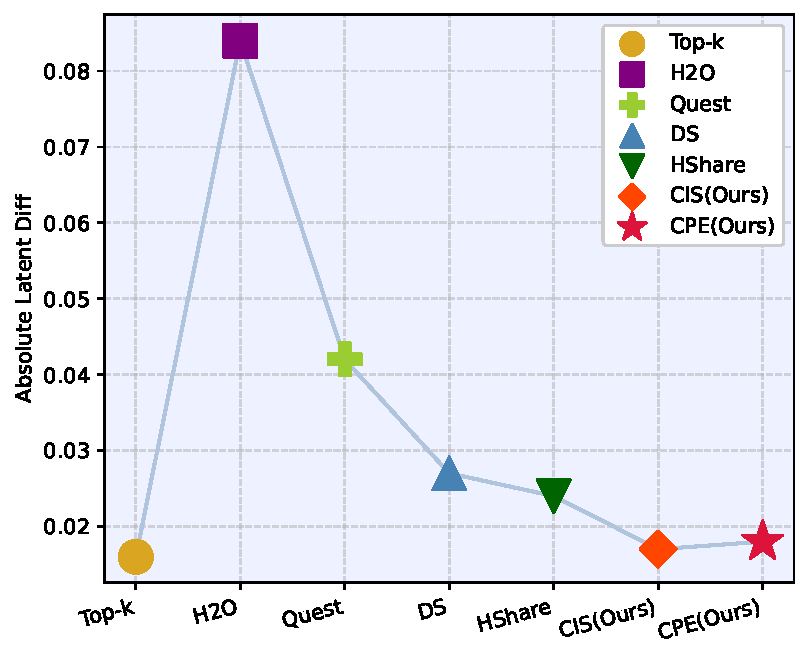
\includegraphics[width=0.305\textwidth]{assets/teaser/latent_diff.pdf}
  }\hfill
  \subfloat[Overall comparisons on accuracy-consumption trade-offs among state-of-the-art baselines.]{
  \footnotesize
  \label{fig:teaser_overall_comp}
    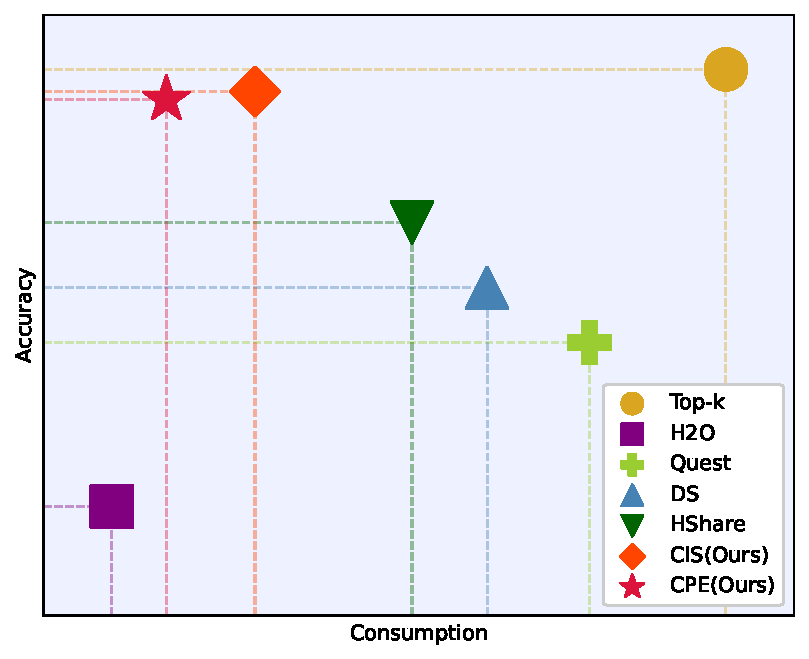
\includegraphics[width=0.305\textwidth]
    {assets/teaser/overall_comp.pdf}
  }
  \vspace{-0.05in}
  \caption{\textbf{Overall analysis of performance and efficiency}. Across induced attention-approximation error and accuracy-efficiency trade-offs, our method consistently surpasses prior SOTA approaches and closely tracks the top-$k$ oracle for optimal KV compression accuracy.}
  \label{fig:teaser}
  \vspace{-0.1in}
\end{figure*}





\iffalse
\begin{figure*}[!t]
    \centering
    \subfigure[Overall comparisons on accuracy and resource consumption among existing techniques.]{
        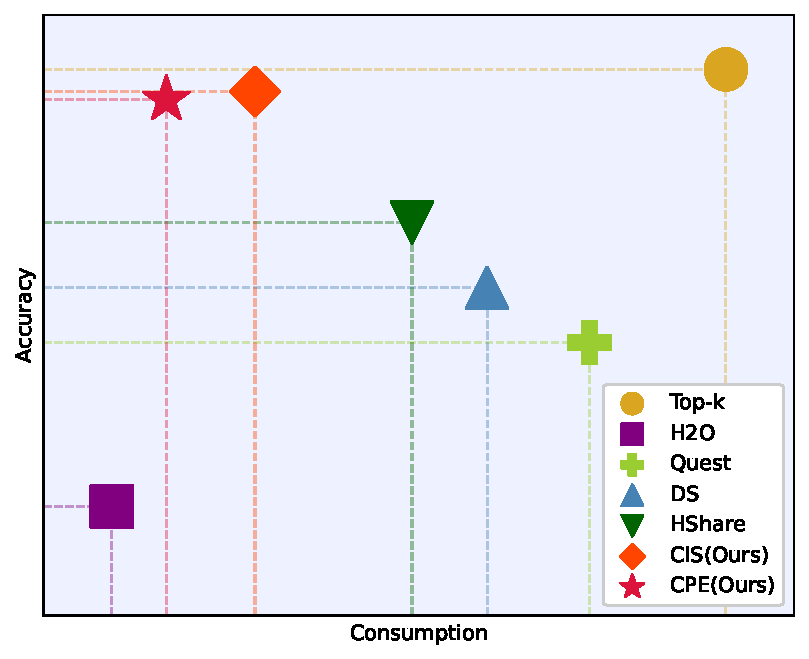
\includegraphics[width=0.305\textwidth]{assets/teaser/overall_comp.pdf}
        %\label{fig:teaser_overall_comp}
    }
    \hfill
    \subfigure[Introduced attention disturbances after filtering attention lgits $<0$.]{
        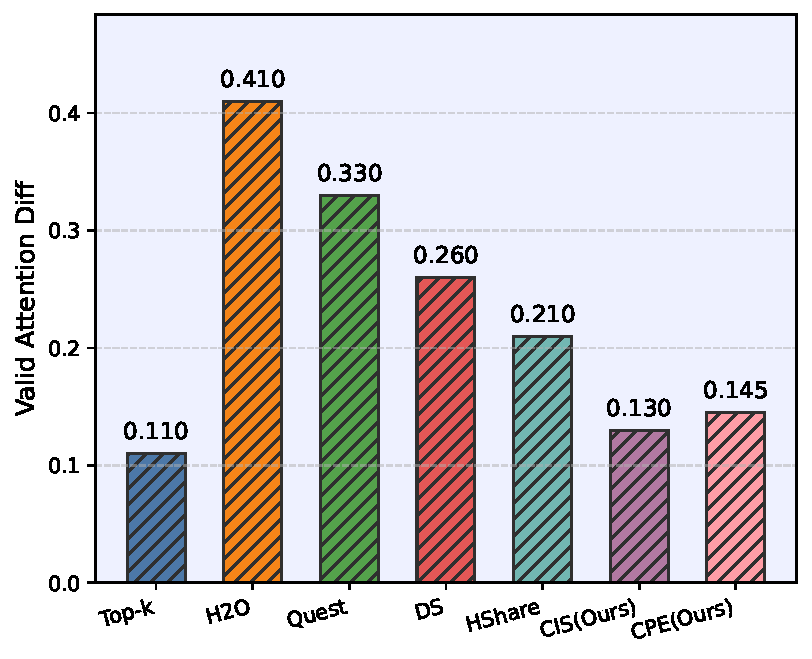
\includegraphics[width=0.305\textwidth]{assets/teaser/attn_diff.pdf}
        %\label{fig:teaser_ppl_elim}
    }
    \hfill
    \subfigure[Introduced absolute differences between original attention outputs.]{
        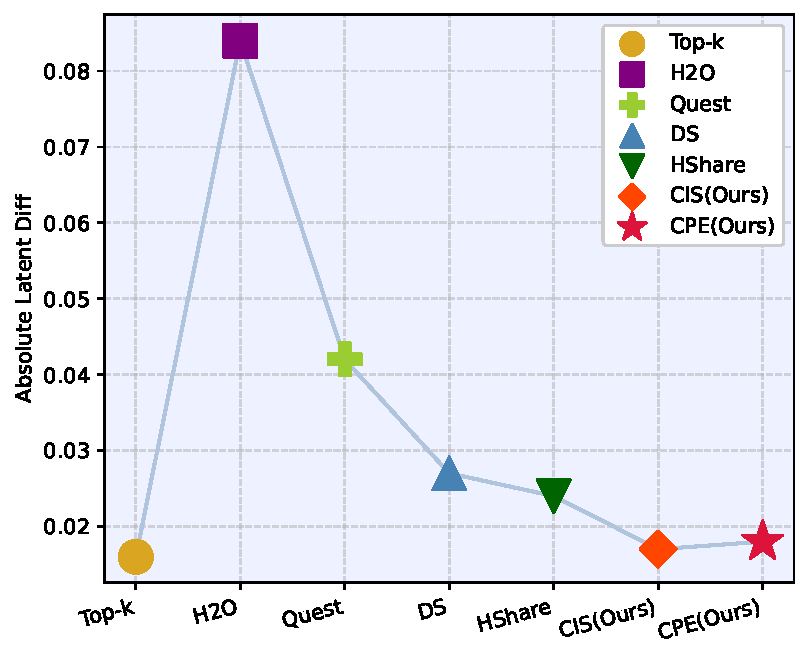
\includegraphics[width=0.305\textwidth]{assets/teaser/latent_diff.pdf}
        % \label{fig:teaser_acc_elim}
    }
    \vspace{-0.1in}
    \caption{Analysis of attention sparsity and its impact. (a) Attention is highly sparse across layers. (b) Perplexity maintains stable when large amounts of low-magnitude attention are eliminated. (c) Accuracy remains robust to large-scale attention pruning.}
    \label{fig:teaser}
    \vspace{-0.1in}
\end{figure*}
\fi




\iffalse
%------------------------------------------------------
\begin{figure*}[!t]
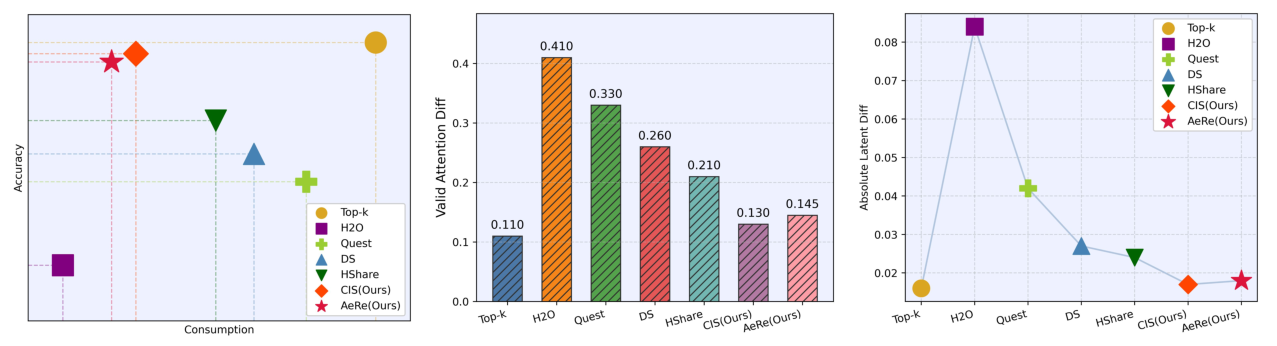
\includegraphics[width=1\textwidth]{assets/Teaser.pdf}
\centering
%\vspace{-1em}
    \caption{\textbf{Distribution of critical indices across heads and layers in LLaMA2-Chat-7B.} We highlight the critical indices in \textcolor{red}{red} and select the critical clusters (\textcolor{green!60!black}{green circles}, without local key tokens) within a range of consecutive queries (\textcolor{violet}{purple box}). Although not strictly contiguous, the critical key indices consistently form stable and dense clusters across multiple heads and layers.}
    \label{fig:teaser}
    %\vspace{-1.5em}
\end{figure*}
%------------------------------------------------------
\fi

Therefore, in this paper, we analyze selection through a \emph{marginal-to–mutual-information} lens and devise a new framework, \textbf{Pre-hoc Sparsity} (PrHS).
Let $\delta$ denote the dropped attention mass (mass of discarded KV entries),
and let $\Delta H$ quantify the induced perturbation of the attention distribution.
We prove that the selection-induced \emph{mutual-information loss} admits an
upper bound that depends only on $\delta$ (Eq.~\eqref{eq:prhs_bound}).
This provides an a-priori error certificate: by constraining $\delta$
before scoring, PrHS instantiates selectors that avoid posterior bias and delivers explicit selection–error control by enforcing conditions that tighten the bound. Consequently, PrHS markedly reduces attention- and output-level perturbations and approaches the oracle frontier in the accuracy–efficiency trade-off (Fig.~\ref{fig:teaser_overall_comp}).
We further quantify deviation from the oracle by $\beta_{\mathrm{th}}$, the
marginal-entropy gap between PrHS and top-$k$; as $\beta_{\mathrm{th}}\!\to\!0$,
PrHS converges to the oracle (Eq.~\ref{eq:limit_to_oracle}; proof in
Sec.~\ref{sec:app_mib_tsa}).



We instantiate three PrHS techniques, Clustered Index Sharing (CIS), Progressive Sliding Attention Window (PSAW), and Early Token Freezing (ETF), each translating a distinct sparsity prior into a PrHS selector. These selectors are then parameterized to tighten the MI upper bound on marginal-entropy error (Eq.~\eqref{eq:prhs_bound}). CIS explores temporal-locality~\cite{wuhshare}: consecutive queries are highly similar. It shares the retrieved set from the top-$k$ oracle across temporally adjacent queries whose embeddings exceed a cosine-similarity threshold, and dilates it by adding neighbors around highest-score indices. PSAW leverages the recency prior~\cite{xiao2023streamingllm,zhang2023h2o}—attention mass concentrates on a local window—and applies a depth-adaptive sliding window that shrinks monotonically with depth, incrementally pruning the candidate KV entries. ETF exploits cross-layer redundancy~\cite{liu2405minicache}: adjacent layers exhibit high KV similarity. ETF freezes stable early tokens to reduce updates. The three selectors act along different axes—time (CIS), depth (PSAW), and layer (ETF)—and compose naturally: CIS seeds the candidate pool with a small budget, then PSAW and ETF intersect their selections with the CIS seed using larger budgets to further prune. Finally, we implement custom CUDA kernels that parallelize index manipulation and sparse-attention computation to minimize runtime overhead. We refer to the combined system as \textbf{CPE}. 

%  relative to state-of-the-art baselines

% within a fixed index radius 

Collectively, CPE delivers competitive reductions in memory footprint and end-to-end latency with substantially improved relative to state-of-the-art (SOTA) baselines (Fig.~\ref{fig:teaser_overall_comp}). Empirically, on LLaMA~\cite{touvron2023llama} and Mistral model families~\cite{jiang2023mistral7b} across GSM8K and CoQA, CIS matches the accuracy of recent SOTA method HShare~\cite{wuhshare} while using only \emph{one-third} of its retrieval complexity. Overall, CPE maintains comparable model quality even with reducing $> \!90\%$ KV-retrieval overhead, while lowering $\sim \! 15\%$ attention FLOPs than prior sparse baselines. On NVIDIA A800-80GB GPUs, CPE attains a $\mathbf{9.9\!\times}$ speedup in attention-operator latency and a $\mathbf{2.8\!\times}$ throughput improvement over original models. Ablation studies in Sec.~\ref{sec:hyper-tune} further confirm that each component contributes reliably. Our contributions are summarized as follows:
\begin{enumerate}[label=\arabic*)]
    \item Rigorous analyses of the mutual information bound from the marginal entropy in KV compression and introduction of Pre-hoc Sparsity towards the accuracy of top-$k$ oracle.
    \item Introduction of CIS, which sustains stable performance at high sharing ratios, together with PSAW and ETF for lossless sparsification of attention computation, all implemented with customized CUDA kernels for parallelization.
    \item Extensive experiments and ablations demonstrating consistent improvements in accuracy, efficiency, and throughput over state-of-the-art baselines.
\end{enumerate}


% We instantiate three PrHS techniques, each with distilled properties from a distinct prior and parameterized to reduce the MI upper bound on marginal-entropy error (Eq.~\eqref{eq:prhs_bound}). Clustered Index Sharing (CIS) explores temporal locality—consecutive queries are highly similar~\cite{wuhshare}—from which we obtain that their most critical entries (positions) cluster (Fig.~\ref{fig:idx_cluster}) and undergo small centroid shifts. CIS shares the critical-index set across temporally adjacent, semantically similar queries (measured by cosine similarity of query embeddings). To preserve recall under shifts, we dilate each shared set by including neighbors within a fixed index radius around highest-score indices, ensuring coverage while enabling aggressive sharing. Progressive Sliding Attention Window (PSAW) leverages the recency prior~\cite{xiao2023streamingllm,zhang2023h2o}: attention mass concentrates on a local window; and the useful tokens shrink with layer depth. PSAW applies a depth-adaptive sliding window that shrinks monotonically with depth, incrementally pruning the candidate set. Building on PSAW, Early Token Freezing (ETF) exploits cross-layer redundancy prior: adjacent layers exhibit high KV similarity~\cite{liu2405minicache}. ETF freezes updates to early tokens once stability criteria are met, further reducing computation and complementing PSAW's incremental pruning. All three techniques are orthogonal and, with appropriately chosen budgets, satisfy the pre-hoc MI bound on approximation error. At inference time, we first apply CIS with a small budget, then apply PSAW and ETF with larger budgets and intersect their selections with CIS to further prune. We implement custom CUDA kernels that parallelize index manipulation and sparse-attention computation to minimize runtime overhead. We refer to the combined system as \textbf{CPE}.


% To championing top-k oracle, we devise a new method, which comprises three complementary techniques. First, noting that critical tokens cluster (\emph{sink effect}, Fig.~\ref{fig:idx_cluster}) and that adjacent queries exhibit \emph{mean-shift} in their critical sets, we propose \textbf{Clustered Index Sharing} (CIS). CIS shares critical indices among semantically similar (measured by cosine similarity in the feature space), temporally adjacent queries. To preserve recall, each shared set is expanded by a fixed index radius to cover local neighbors, yielding near-complete cluster coverage to avoid omission of critical indices, sustaining accuracy under aggressive sharing. Nest, exploiting \emph{progressive information propagation} of LLMs, we introduce \textbf{Progressive Sliding Attention Window} (PSAW) and \textbf{Early Token Freezing} (ETF) to incrementally prune redundant attention with increasing layer depth. Finally, we pair these algorithms with customized CUDA kernels that parallelize index manipulation and sparse-attention computation, minimizing runtime overhead. We refer to the combined system as \textbf{CPE}.

